%!TEX program = xelatex
% This is a simple sample document.  For more complicated documents take a look in the exercise tab. Note that everything that comes after a % symbol is treated as comment and ignored when the code is compiled.
\documentclass{mancls}% \documentclass{} is the first command in any LaTeX code.  It is used to define what kind of document you are creating such as an article or a book, and begins the document preamble
\usepackage{longtable} % \usepackage is a command that allows you to add functionality to your LaTeX code
\usepackage{amsmath} % \usepackage is a command that allows you to add functionality to your LaTeX code
\title{Purrfect Eats APP V1.0}
\author{麻靓靓} % Sets authors name
%\date{\today} % Sets date for date compiled

% The preamble ends with the command \begin{document}
\begin{document} % All begin commands must be paired with an end command somewhere
\section*{文 件 修 订 记 录}
\addcontentsline{toc}{section}{文 件 修 订 记 录}


% 使用longtable环境创建一个整页表格
\begin{longtable}{|c|c|c|c|}
  \hline
  \textbf{版本号} & \textbf{生成日期} & \textbf{作者} & \textbf{修订内容} \\
  \hline
  V1.0         & 2024-4-25     & 麻靓靓         & 初始版本          \\
  \hline
               &               &             &               \\
  \hline
               &               &             &               \\
  \hline
               &               &             &               \\
  \hline
               &               &             &               \\
  \hline
               &               &             &               \\
  \hline
               &               &             &               \\
  \hline
               &               &             &               \\
  \hline
               &               &             &               \\
  \hline
               &               &             &               \\
  \hline
               &               &             &               \\
  \hline
               &               &             &               \\
  \hline
               &               &             &               \\
  \hline
               &               &             &               \\
  \hline
               &               &             &               \\
  \hline
               &               &             &               \\
  \hline
\end{longtable}
\pagebreak

\section{总体功能描述}


我们的软件是一款名为“Purrfect Eats APP”的点击游戏,旨在通过玩家的点击操作帮助小猫经营餐厅以赚取金钱。游戏采用三层结构,使用主流的 Unity 引擎进行开发。

在游戏中,玩家需要不断点击以帮助小猫制作和出售菜品,从而赚取金钱。通过积累的金钱,玩家可以升级菜品,提高餐厅的效率和盈利能力。此外,玩家还可以招募经理来自动化部分餐厅的运营,进一步提升游戏体验和经营效果。

游戏开始之后,玩家将进入餐厅的经营界面,通过点击操作来制作和出售菜品。随着游戏进程,玩家可以解锁更多的菜品和经理,逐步提升餐厅的等级和成就。

\pagebreak

% 运行环境
\section{运行环境}
\subsection{硬件要求}
\begin{longtable}{|c|c|}
  %\hline
  %\multicolumn{2}{|c|}{\textbf{硬件要求}} \\
  \hline
  类别  & 基本要求                     \\
  \hline
  客户端 & iOS设备,1G内存及以上;存储空间40M及以上 \\
  \hline
  客户端 & 小程序平台,1G内存及以上;存储空间40M及以上 \\
  \hline
\end{longtable}

\vspace{1cm}

\subsection{软件要求}
% 软件要求表格
\begin{longtable}{|c|c|c|}
  %\hline
  %\multicolumn{3}{|c|}{\textbf{软件要求}}         \\
  \hline
  类别  & 名称   & 基本环境             \\
  \hline
  客户端 & 操作系统 & iOS 10.0及以上版本    \\
  \hline
  客户端 & 操作系统 & 微信小程序,微信版本7.0及以上 \\
  \hline
\end{longtable}
\pagebreak
\section{软件编译环境}

\subsection{编译工具}

我们使用Unity 2022.1.13作为主要的开发和编译工具。Unity是一款功能强大的跨平台游戏引擎,支持2D和3D游戏的开发,并且提供了丰富的开发工具和资源,适用于各种类型的游戏开发。

\subsection{操作系统}

\begin{itemize}
  \item \textbf{Windows}:Windows 10及以上版本
  \item \textbf{macOS}:macOS 10.15及以上版本
\end{itemize}

\subsection{其他依赖}

\begin{itemize}
  \item \textbf{Visual Studio}:推荐使用Visual Studio 2019或更高版本,带有Unity工具插件。
  \item \textbf{Xcode}:对于iOS平台的开发,需安装Xcode 12.5及以上版本。
  \item \textbf{微信开发者工具}:用于调试和发布微信小程序,需安装最新版微信开发者工具。
\end{itemize}

\subsection{环境配置}

\begin{enumerate}
  \item \textbf{安装Unity}:从Unity官方下载安装Unity Hub,并通过Unity Hub安装Unity 2022.1.13版本。
  \item \textbf{设置开发环境}:
        \begin{itemize}
          \item 打开Unity Hub,创建或打开项目。
          \item 在项目设置中,配置iOS和微信小程序的相关参数。
        \end{itemize}
  \item \textbf{安装依赖工具}:
        \begin{itemize}
          \item 下载并安装Visual Studio,确保勾选Unity工具插件。
          \item 对于iOS开发,确保安装并配置好Xcode。
          \item 下载并安装微信开发者工具,并在微信开发者工具中配置好项目路径。
        \end{itemize}
\end{enumerate}

\subsection{项目构建}

\subsubsection{iOS平台}

\begin{enumerate}
  \item 在Unity中选择\texttt{File > Build Settings}。
  \item 选择\texttt{iOS}平台,并点击\texttt{Switch Platform}。
  \item 配置\texttt{Player Settings},确保填写正确的包名和其他信息。
  \item 点击\texttt{Build},生成Xcode项目文件。
  \item 打开Xcode项目文件,配置签名证书并进行编译。
\end{enumerate}

\subsubsection{微信小程序平台}

\begin{enumerate}
  \item 在Unity中安装微信小程序插件(例如:使用第三方插件如WeChat Minigame SDK)。
  \item 配置插件的相关参数。
  \item 在\texttt{Build Settings}中选择微信小程序平台,并点击\texttt{Switch Platform}。
  \item 点击\texttt{Build},生成微信小程序项目文件。
  \item 打开微信开发者工具,导入生成的项目文件并进行调试和发布。
\end{enumerate}

通过上述步骤配置和使用软件编译环境,可以确保项目在iOS和微信小程序平台上的顺利开发和发布。
\pagebreak

\section{软件安装说明}

\subsection{iOS平台}

\begin{enumerate}
  \item \textbf{从App Store下载}:
        \begin{itemize}
          \item 打开iOS设备上的App Store应用。
          \item 在搜索栏中输入“Purrfect Eats APP”并进行搜索。
          \item 在搜索结果中找到我们的游戏,并点击“获取”按钮进行下载和安装。
        \end{itemize}
  \item \textbf{通过TestFlight测试(仅限测试人员)}:
        \begin{itemize}
          \item 安装TestFlight应用程序(可从App Store下载)。
          \item 通过邀请链接或TestFlight应用中的代码接受测试邀请。
          \item 在TestFlight应用中找到“Purrfect Eats APP”并点击“安装”按钮进行安装。
        \end{itemize}
\end{enumerate}

\subsection{微信小程序平台}

\begin{enumerate}
  \item \textbf{通过微信搜索小程序}:
        \begin{itemize}
          \item 打开微信应用,进入主界面。
          \item 在顶部搜索栏中输入“Purrfect Eats APP”并进行搜索。
          \item 在搜索结果中找到我们的微信小程序,并点击进入。
          \item 选择“添加到我的小程序”以便下次快速访问。
        \end{itemize}
  \item \textbf{通过扫描二维码}:
        \begin{itemize}
          \item 打开微信应用,进入主界面。
          \item 点击右上角的“+”号,选择“扫一扫”功能。
          \item 扫描官方提供的“Purrfect Eats APP”小程序二维码。
          \item 进入小程序后,选择“添加到我的小程序”以便下次快速访问。
        \end{itemize}
\end{enumerate}
\subsection{第一次打开软件}

\begin{itemize}
  \item 第一次打开软件将会进入加载界面,效果如下图所示:
        \begin{figure}[h]
          \centering
          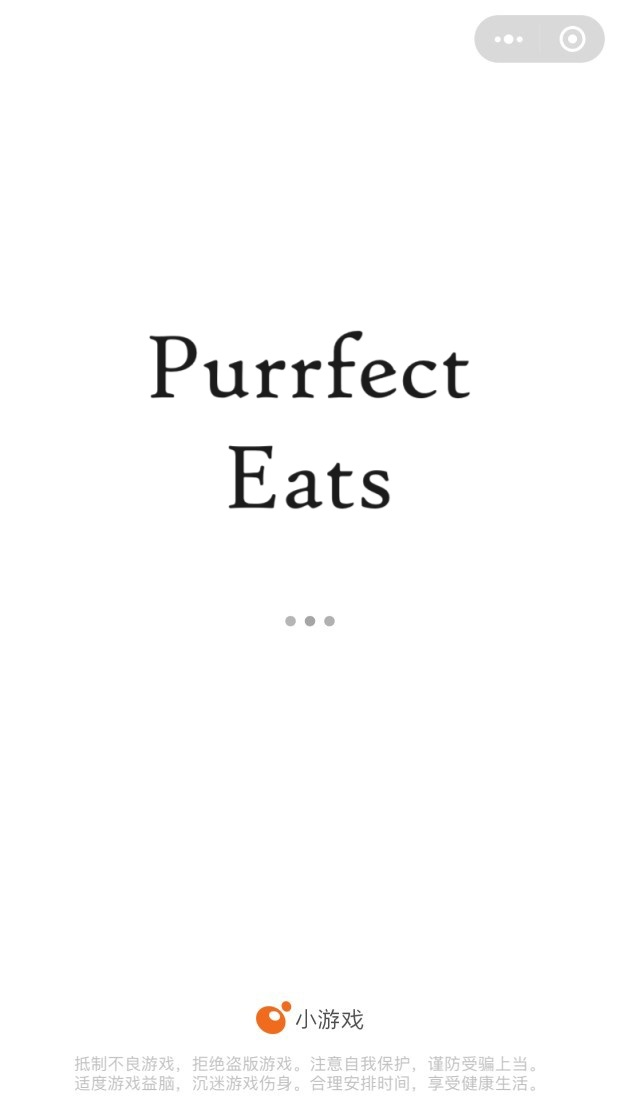
\includegraphics[height=0.6\textheight]{screenshots/minigame.jpg}
          \caption{首次加载界面}
        \end{figure}
\end{itemize}
\subsection{常见问题}

\begin{itemize}
  \item \textbf{无法找到游戏}:
        \begin{itemize}
          \item 确保使用的是最新版本的App Store或微信应用。
          \item 检查拼写是否正确,或者尝试不同的关键词。
        \end{itemize}
  \item \textbf{安装失败}:
        \begin{itemize}
          \item 检查设备的存储空间是否足够。
          \item 确保设备的操作系统版本符合最低要求(iOS 10.0及以上)。
          \item 如果仍有问题,可以尝试重新启动设备或联系客服获取帮助。
        \end{itemize}
\end{itemize}
\pagebreak
\section{游戏启动}

待游戏安装加载完成后,玩家可以在主页选择进入游戏,进行游戏。游戏启动后的页面如图所示:

\begin{figure}[h]
  \centering
  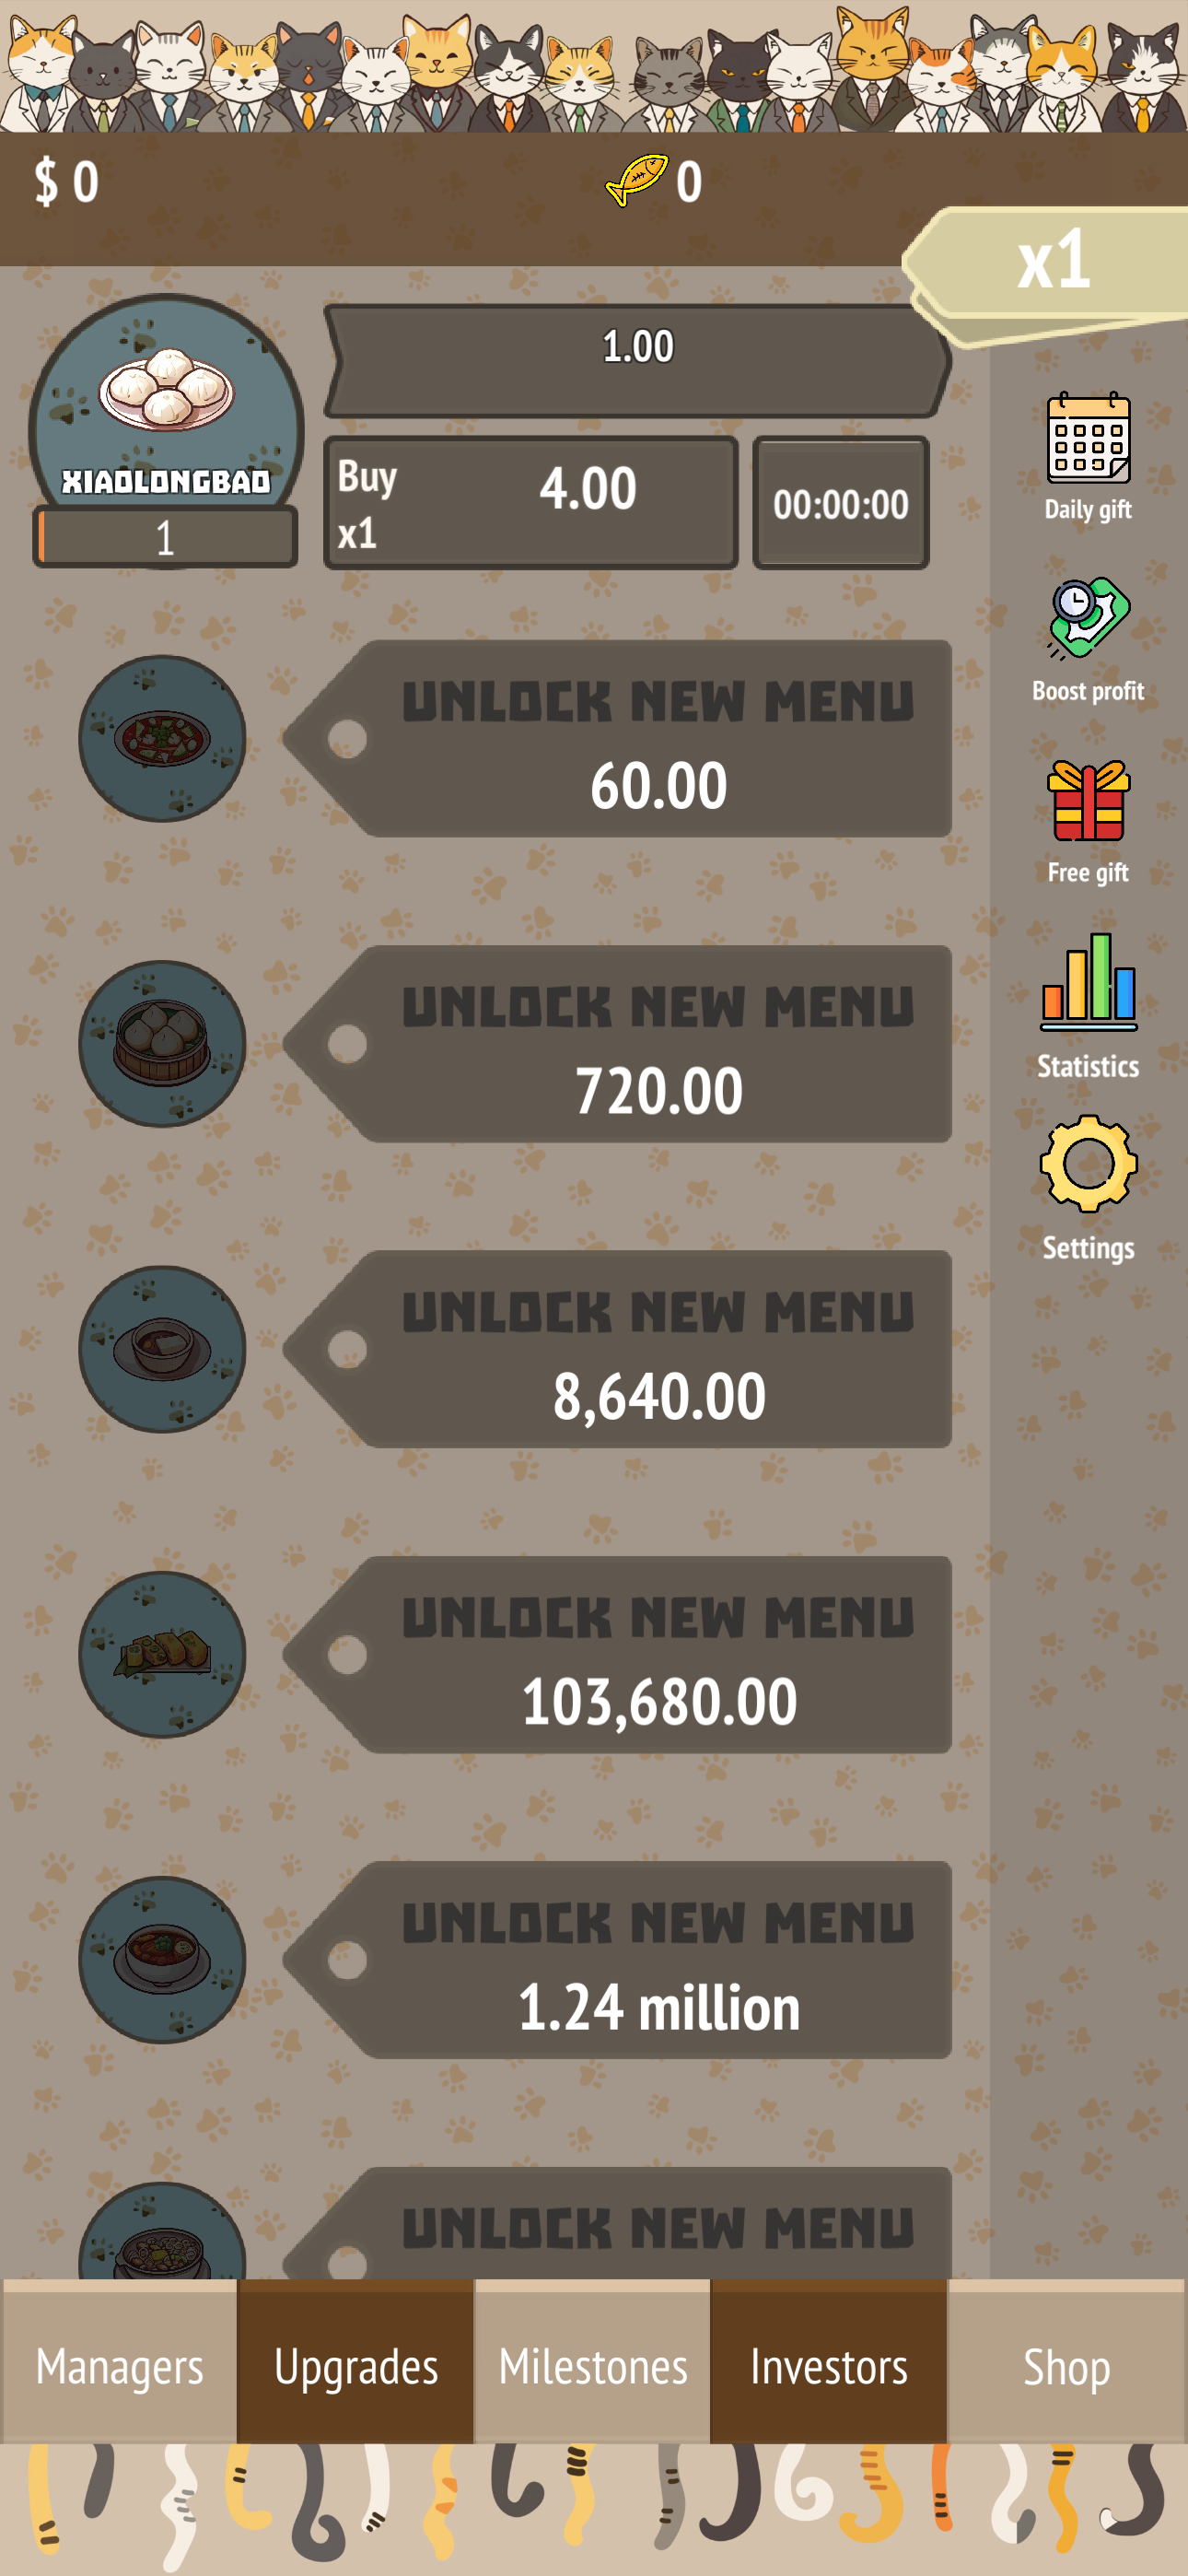
\includegraphics[height=0.6\textheight]{screenshots/PurrfectEats_004.png}
  \caption{游戏启动页面}
\end{figure}

\subsection{游戏启动页面介绍}

\begin{enumerate}
  \item \textbf{顶部显示栏}:
        \begin{itemize}
          \item 显示玩家的当前金钱和鱼币数量。
          \item 玩家点击小猫头像可以查看和管理团队成员。
        \end{itemize}
  \item \textbf{主要操作区域}:
        \begin{itemize}
          \item 当前菜单项的生产情况和单价。
          \item “Buy x1”按钮用于购买或升级当前菜单项。
          \item “Unlock New Menu”按钮用于解锁新菜品,每个菜品都有不同的解锁价格。
        \end{itemize}
  \item \textbf{右侧功能栏}:
        \begin{itemize}
          \item 日常礼包:玩家可以领取每日奖励。
          \item 提升利润:提供临时的收益加成。
          \item 免费礼物:定期赠送免费礼物。
          \item 统计数据:查看当前的经营数据和统计信息。
          \item 设置:访问游戏设置界面。
        \end{itemize}
  \item \textbf{底部导航栏}:
        \begin{itemize}
          \item 管理:玩家可以雇佣和管理经理,自动化餐厅运营。
          \item 升级:升级餐厅的设施和菜品,提升效率和收益。
          \item 里程碑:查看和达成游戏中的成就。
          \item 投资者:与投资者互动,获取额外的资金和支持。
          \item 商店:购买各种游戏内物品和道具,提升游戏体验。
        \end{itemize}
\end{enumerate}

玩家通过点击和互动,可以不断提升餐厅的经营水平,赚取更多的金钱和奖励。

\pagebreak
\section{游戏玩法}

\subsection{基本操作}

在游戏启动后,玩家可以通过点击操作帮助小猫经营餐厅,制作并出售各种菜品,以赚取金钱。游戏的基本操作界面如下:

\begin{figure}[h]
  \centering
  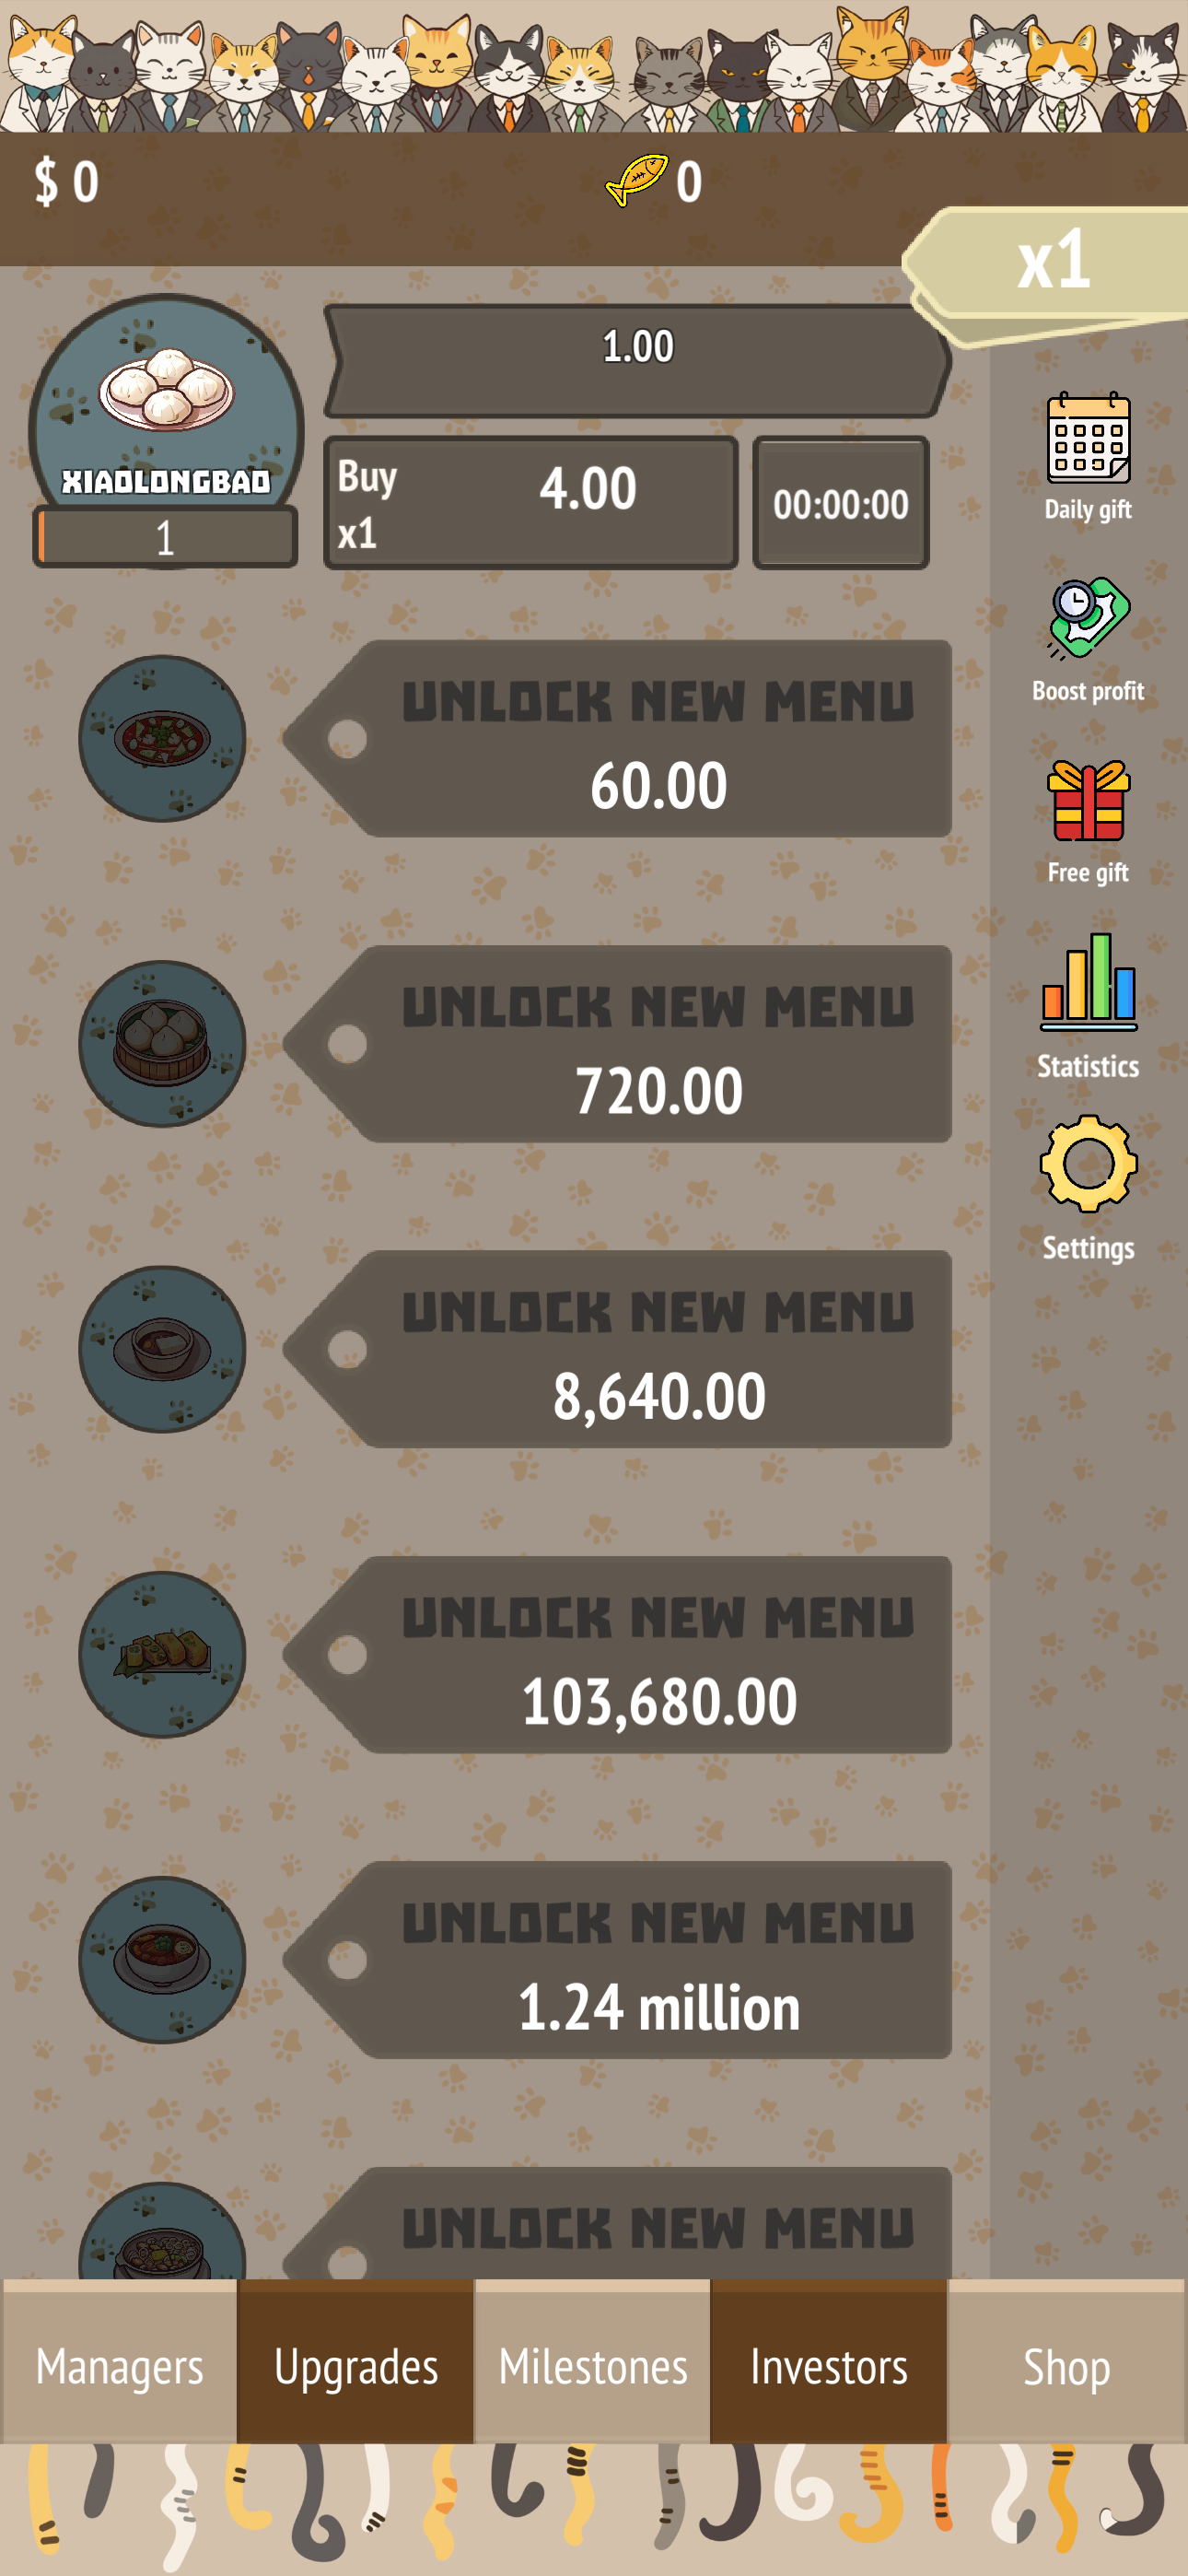
\includegraphics[height=0.6\textheight]{screenshots/PurrfectEats_004.png}
  \caption{游戏启动页面}
\end{figure}

\subsection{经理管理}

玩家可以通过雇佣经理来自动化餐厅的运营,提高效率和收益。每位经理都有特定的任务和能力,雇佣后可以帮助玩家自动制作特定的菜品。经理管理界面如下:

\begin{figure}[h]
  \centering
  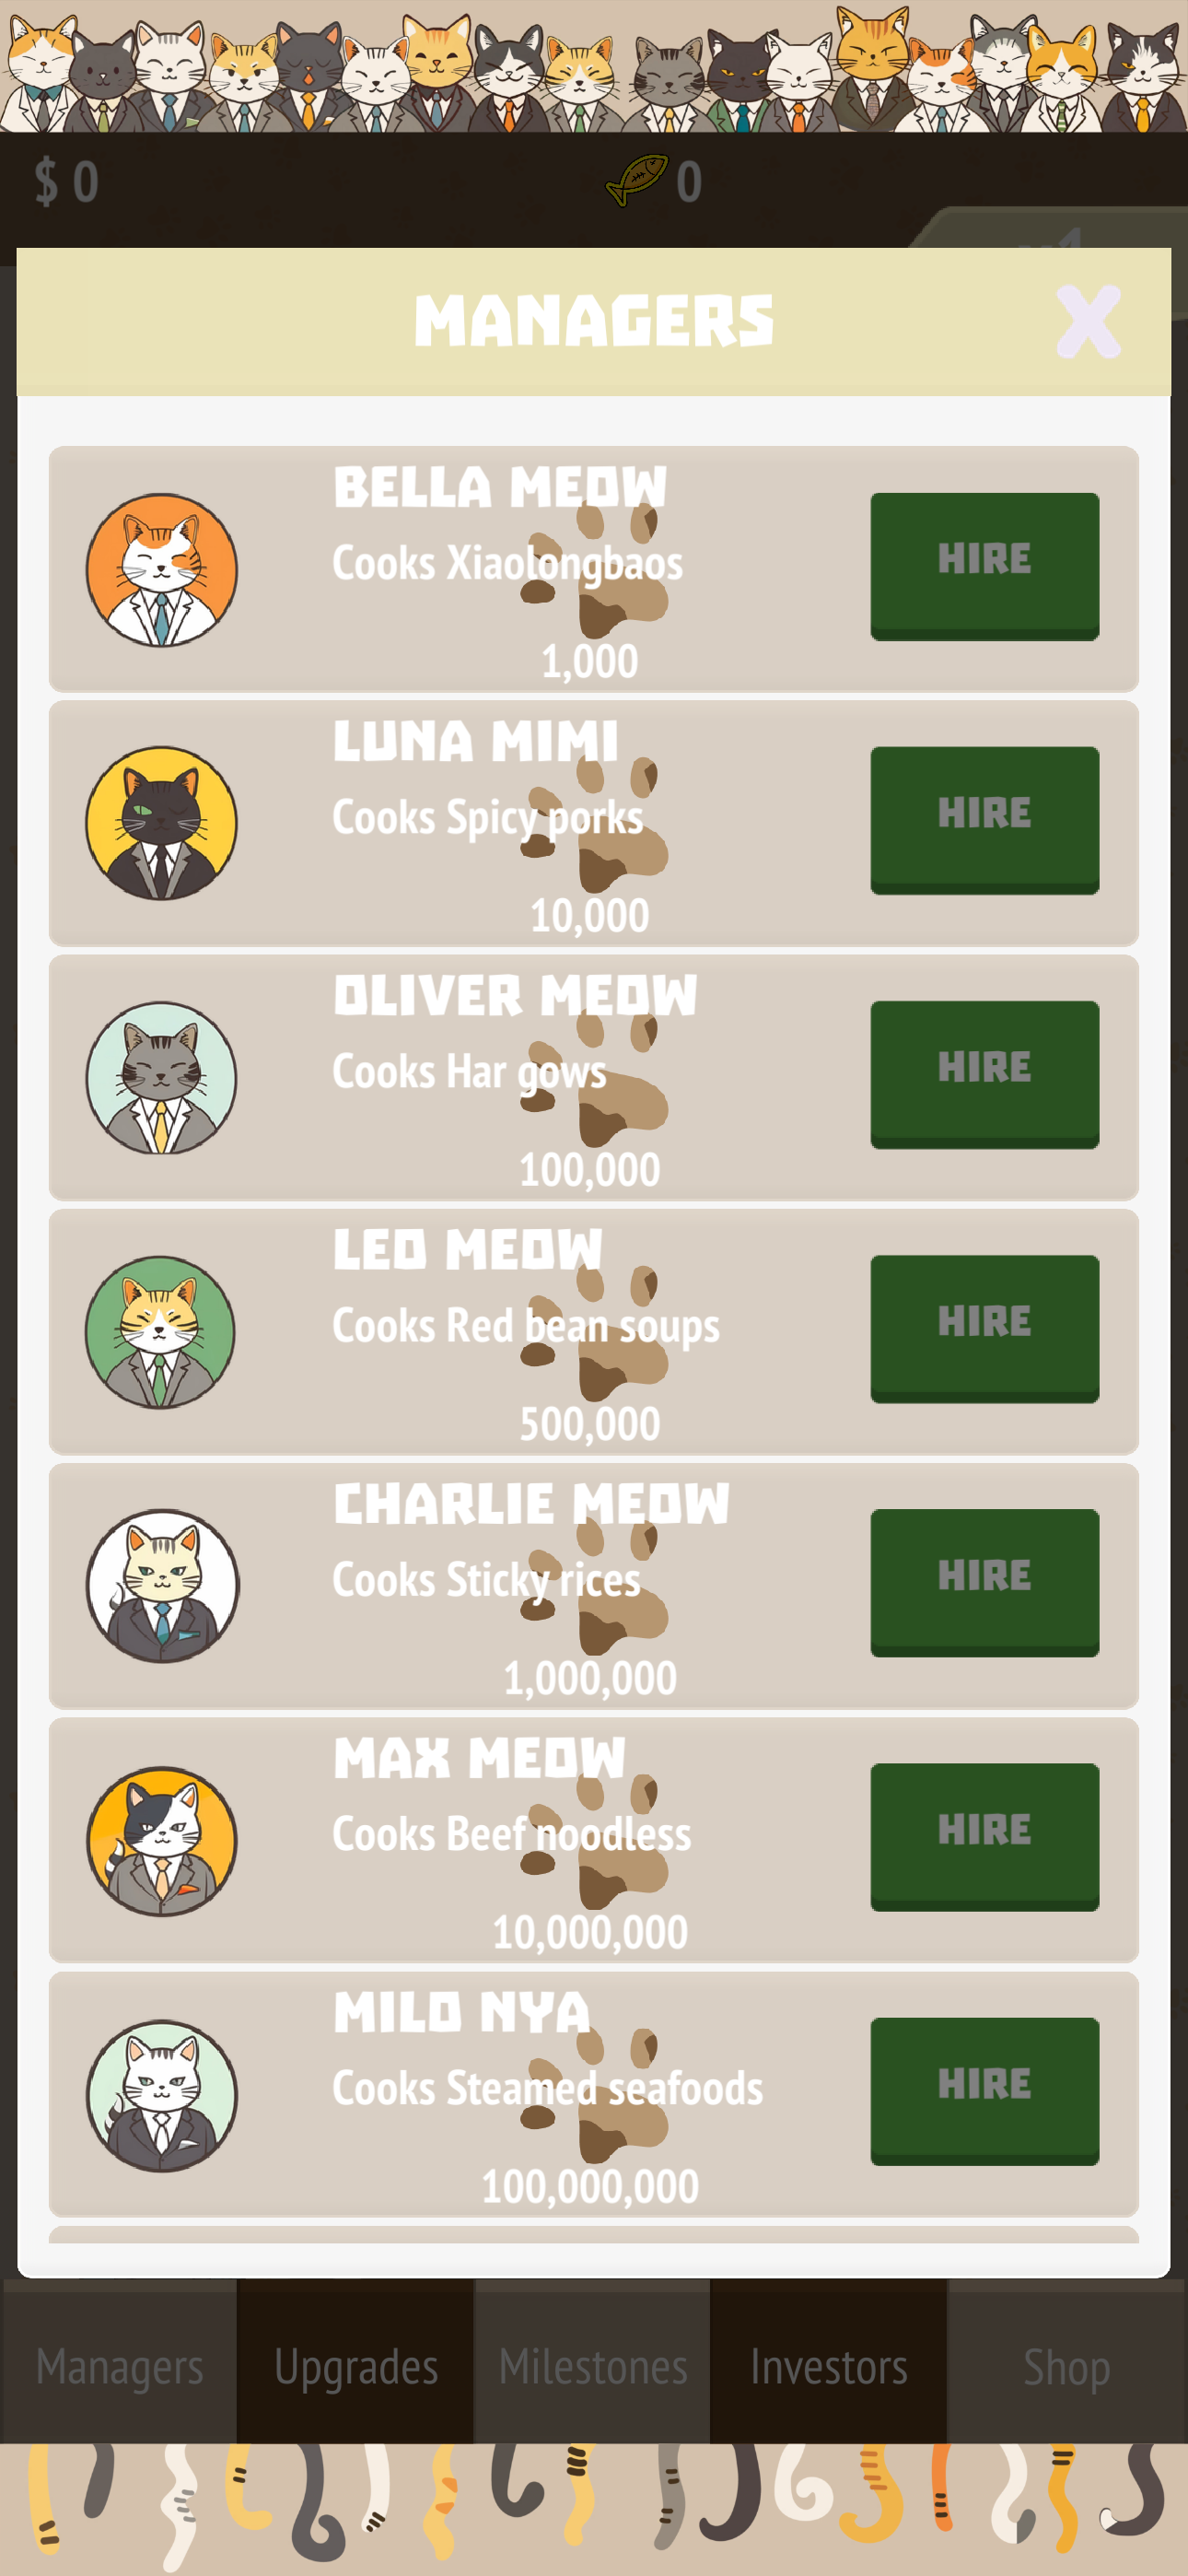
\includegraphics[height=0.6\textheight]{screenshots/PurrfectEats_005.png}
  \caption{经理管理界面}
\end{figure}

\subsubsection{雇佣经理}

在经理管理界面中,玩家可以看到可雇佣的经理列表。每位经理的雇佣费用不同,费用随经理的能力和作用而变化。点击“Hire”按钮即可雇佣相应的经理。

\subsubsection{经理列表}

\begin{itemize}
  \item \textbf{Bella Meow}:负责制作小笼包,雇佣费用为1,000金币。
  \item \textbf{Luna Mimi}:负责制作辣猪肉,雇佣费用为10,000金币。
  \item \textbf{Oliver Meow}:负责制作虾饺,雇佣费用为100,000金币。
  \item \textbf{Leo Meow}:负责制作红豆汤,雇佣费用为500,000金币。
  \item \textbf{Charlie Meow}:负责制作糯米饭,雇佣费用为1,000,000金币。
  \item \textbf{Max Meow}:负责制作牛肉面,雇佣费用为10,000,000金币。
  \item \textbf{Milo Nya}:负责制作蒸海鲜,雇佣费用为100,000,000金币。
\end{itemize}

\subsection{里程碑达成}

玩家在游戏中可以通过达成各种里程碑来获取额外的收益和奖励。里程碑界面如下:

\begin{figure}[h]
  \centering
  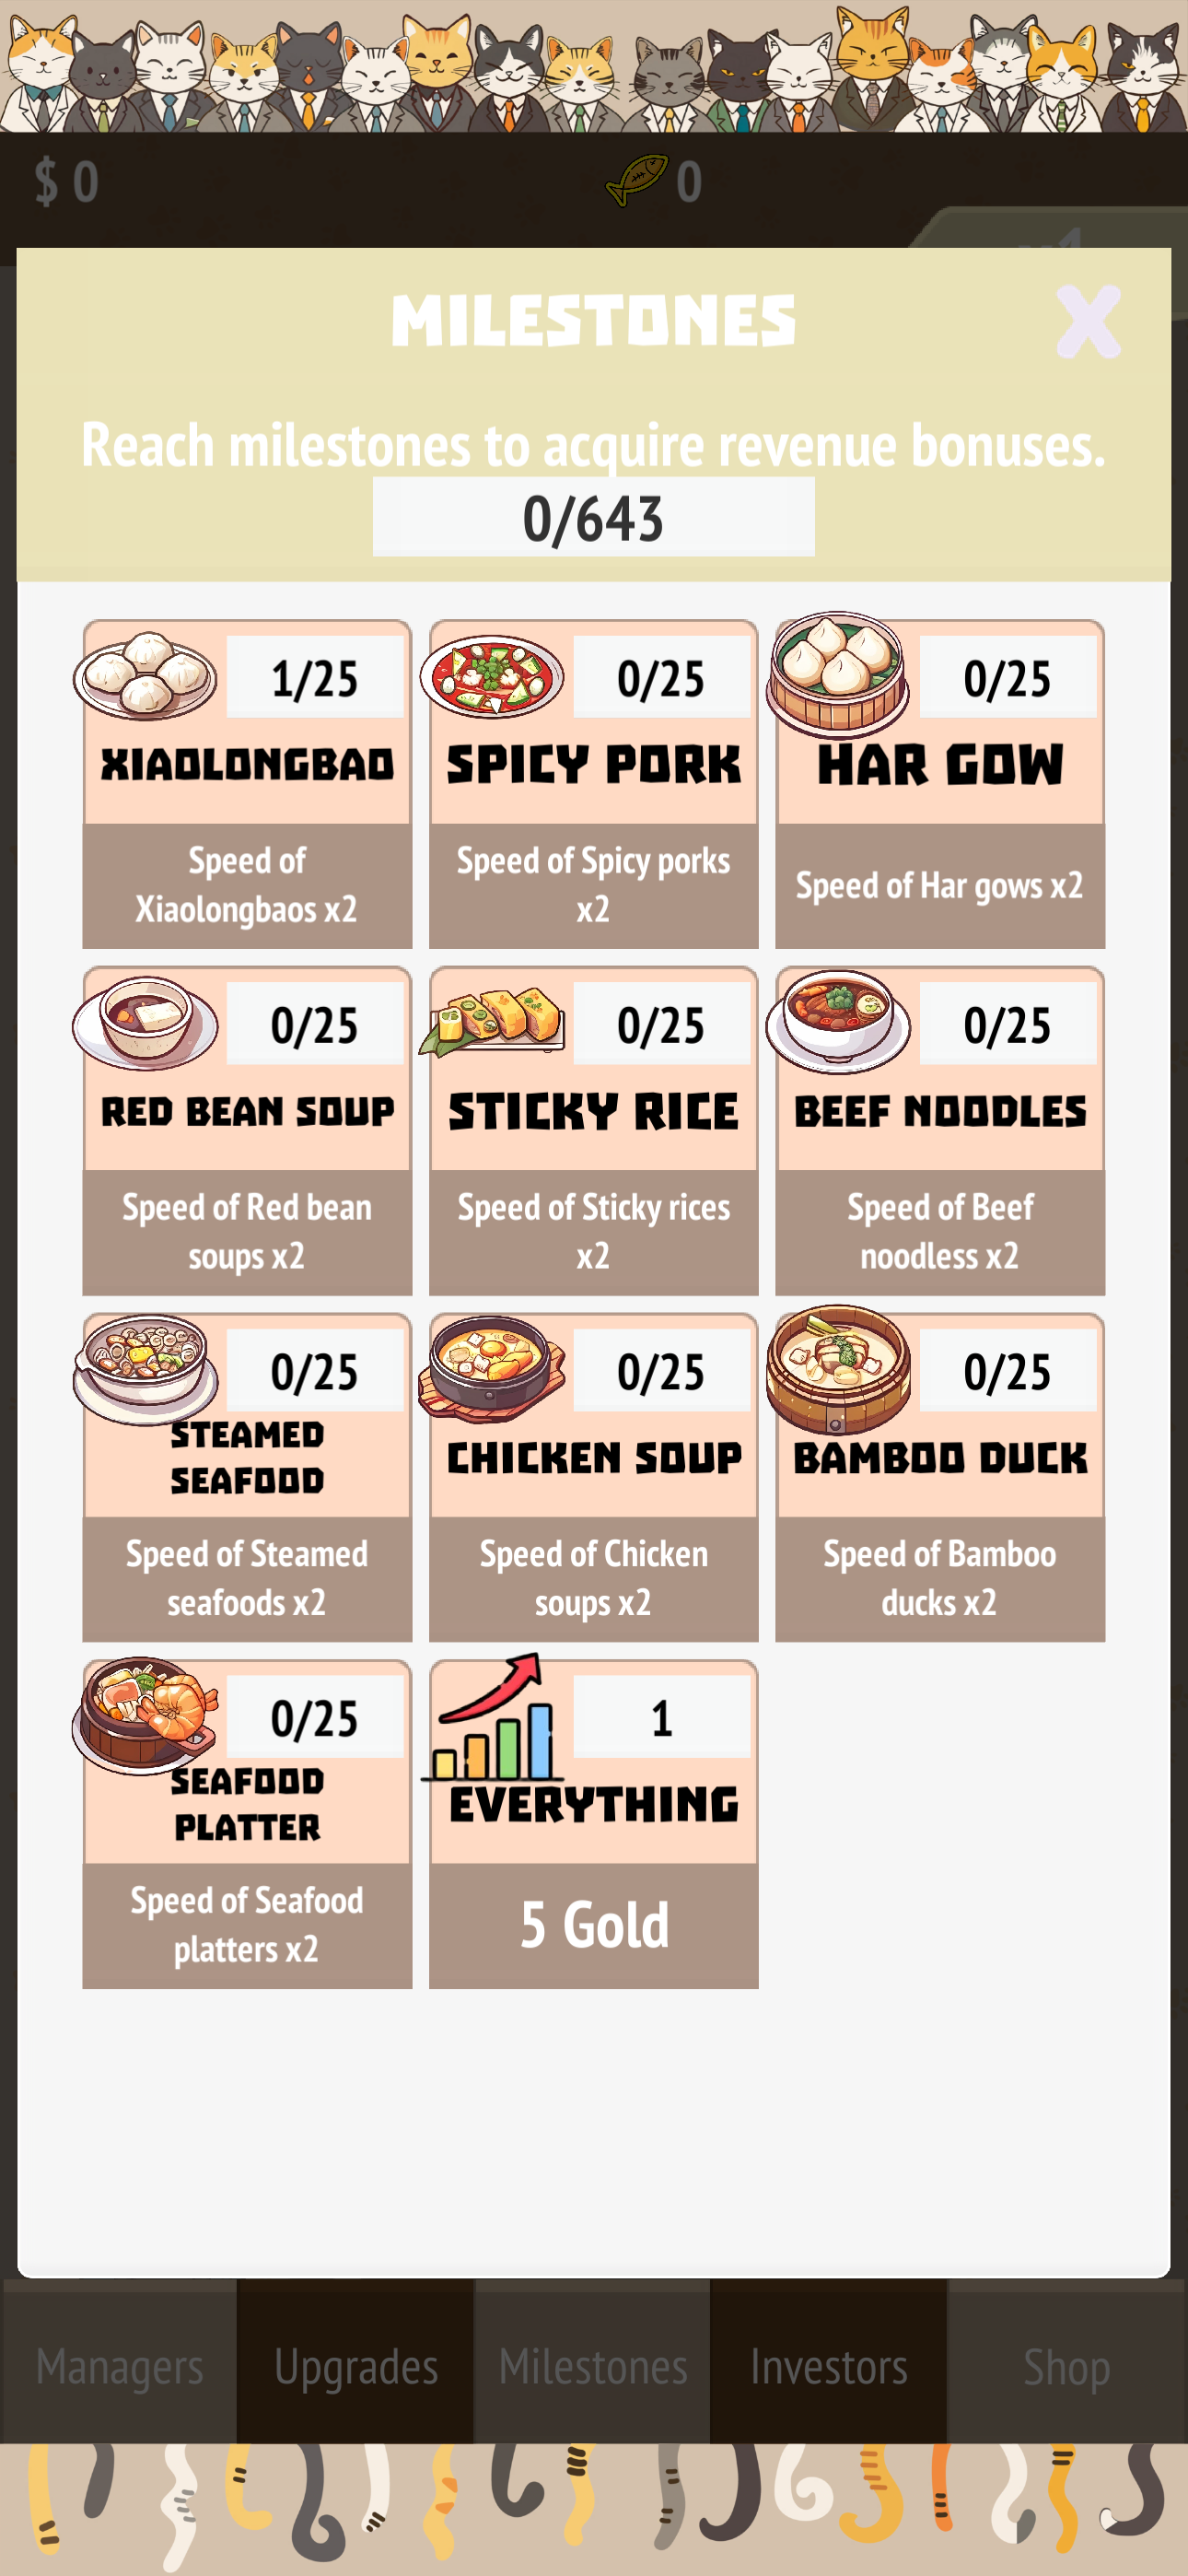
\includegraphics[height=0.6\textheight]{screenshots/PurrfectEats_007.png}
  \caption{里程碑界面}
\end{figure}

\subsubsection{里程碑类型}

不同的菜品有不同的里程碑,每个里程碑都需要玩家达到特定的目标。达成里程碑后,玩家可以获得相应的奖励,如增加菜品制作速度等。

\begin{itemize}
  \item \textbf{小笼包(Xiaolongbao)}:每达成一次里程碑,制作速度翻倍。
  \item \textbf{辣猪肉(Spicy Pork)}:每达成一次里程碑,制作速度翻倍。
  \item \textbf{虾饺(Har Gow)}:每达成一次里程碑,制作速度翻倍。
  \item \textbf{红豆汤(Red Bean Soup)}:每达成一次里程碑,制作速度翻倍。
  \item \textbf{糯米饭(Sticky Rice)}:每达成一次里程碑,制作速度翻倍。
  \item \textbf{牛肉面(Beef Noodles)}:每达成一次里程碑,制作速度翻倍。
  \item \textbf{蒸海鲜(Steamed Seafood)}:每达成一次里程碑,制作速度翻倍。
  \item \textbf{鸡汤(Chicken Soup)}:每达成一次里程碑,制作速度翻倍。
  \item \textbf{竹鸭(Bamboo Duck)}:每达成一次里程碑,制作速度翻倍。
  \item \textbf{海鲜拼盘(Seafood Platter)}:每达成一次里程碑,制作速度翻倍。
  \item \textbf{综合(Everything)}:达到所有菜品的里程碑,可以获得额外的金币奖励。
\end{itemize}

通过不断地点击和互动,升级菜品和设施,雇佣经理以及达成里程碑,玩家可以不断提升餐厅的经营水平,赚取更多的金钱和奖励,体验经营餐厅的乐趣。
\pagebreak
\section{游戏结束}

\subsection{游戏结束条件}

当玩家在游戏中达到某些特定条件时,游戏将会结束。这些条件包括但不限于:
\begin{itemize}
  \item 达到最高级别的餐厅等级
  \item 完成所有里程碑任务
  \item 玩家选择手动结束游戏
\end{itemize}

\subsection{游戏结束后的统计信息}

游戏结束后,将展示玩家的最终得分和经营统计信息,包括:
\begin{itemize}
  \item 总收入
  \item 总花费
  \item 雇佣的经理数量
  \item 解锁的菜品数量
\end{itemize}

\pagebreak

\section{设置界面}

玩家可以通过点击游戏中的“设置”按钮进入设置界面,在这里可以调整游戏的音效和音乐设置。设置界面如下:

\begin{figure}[h]
  \centering
  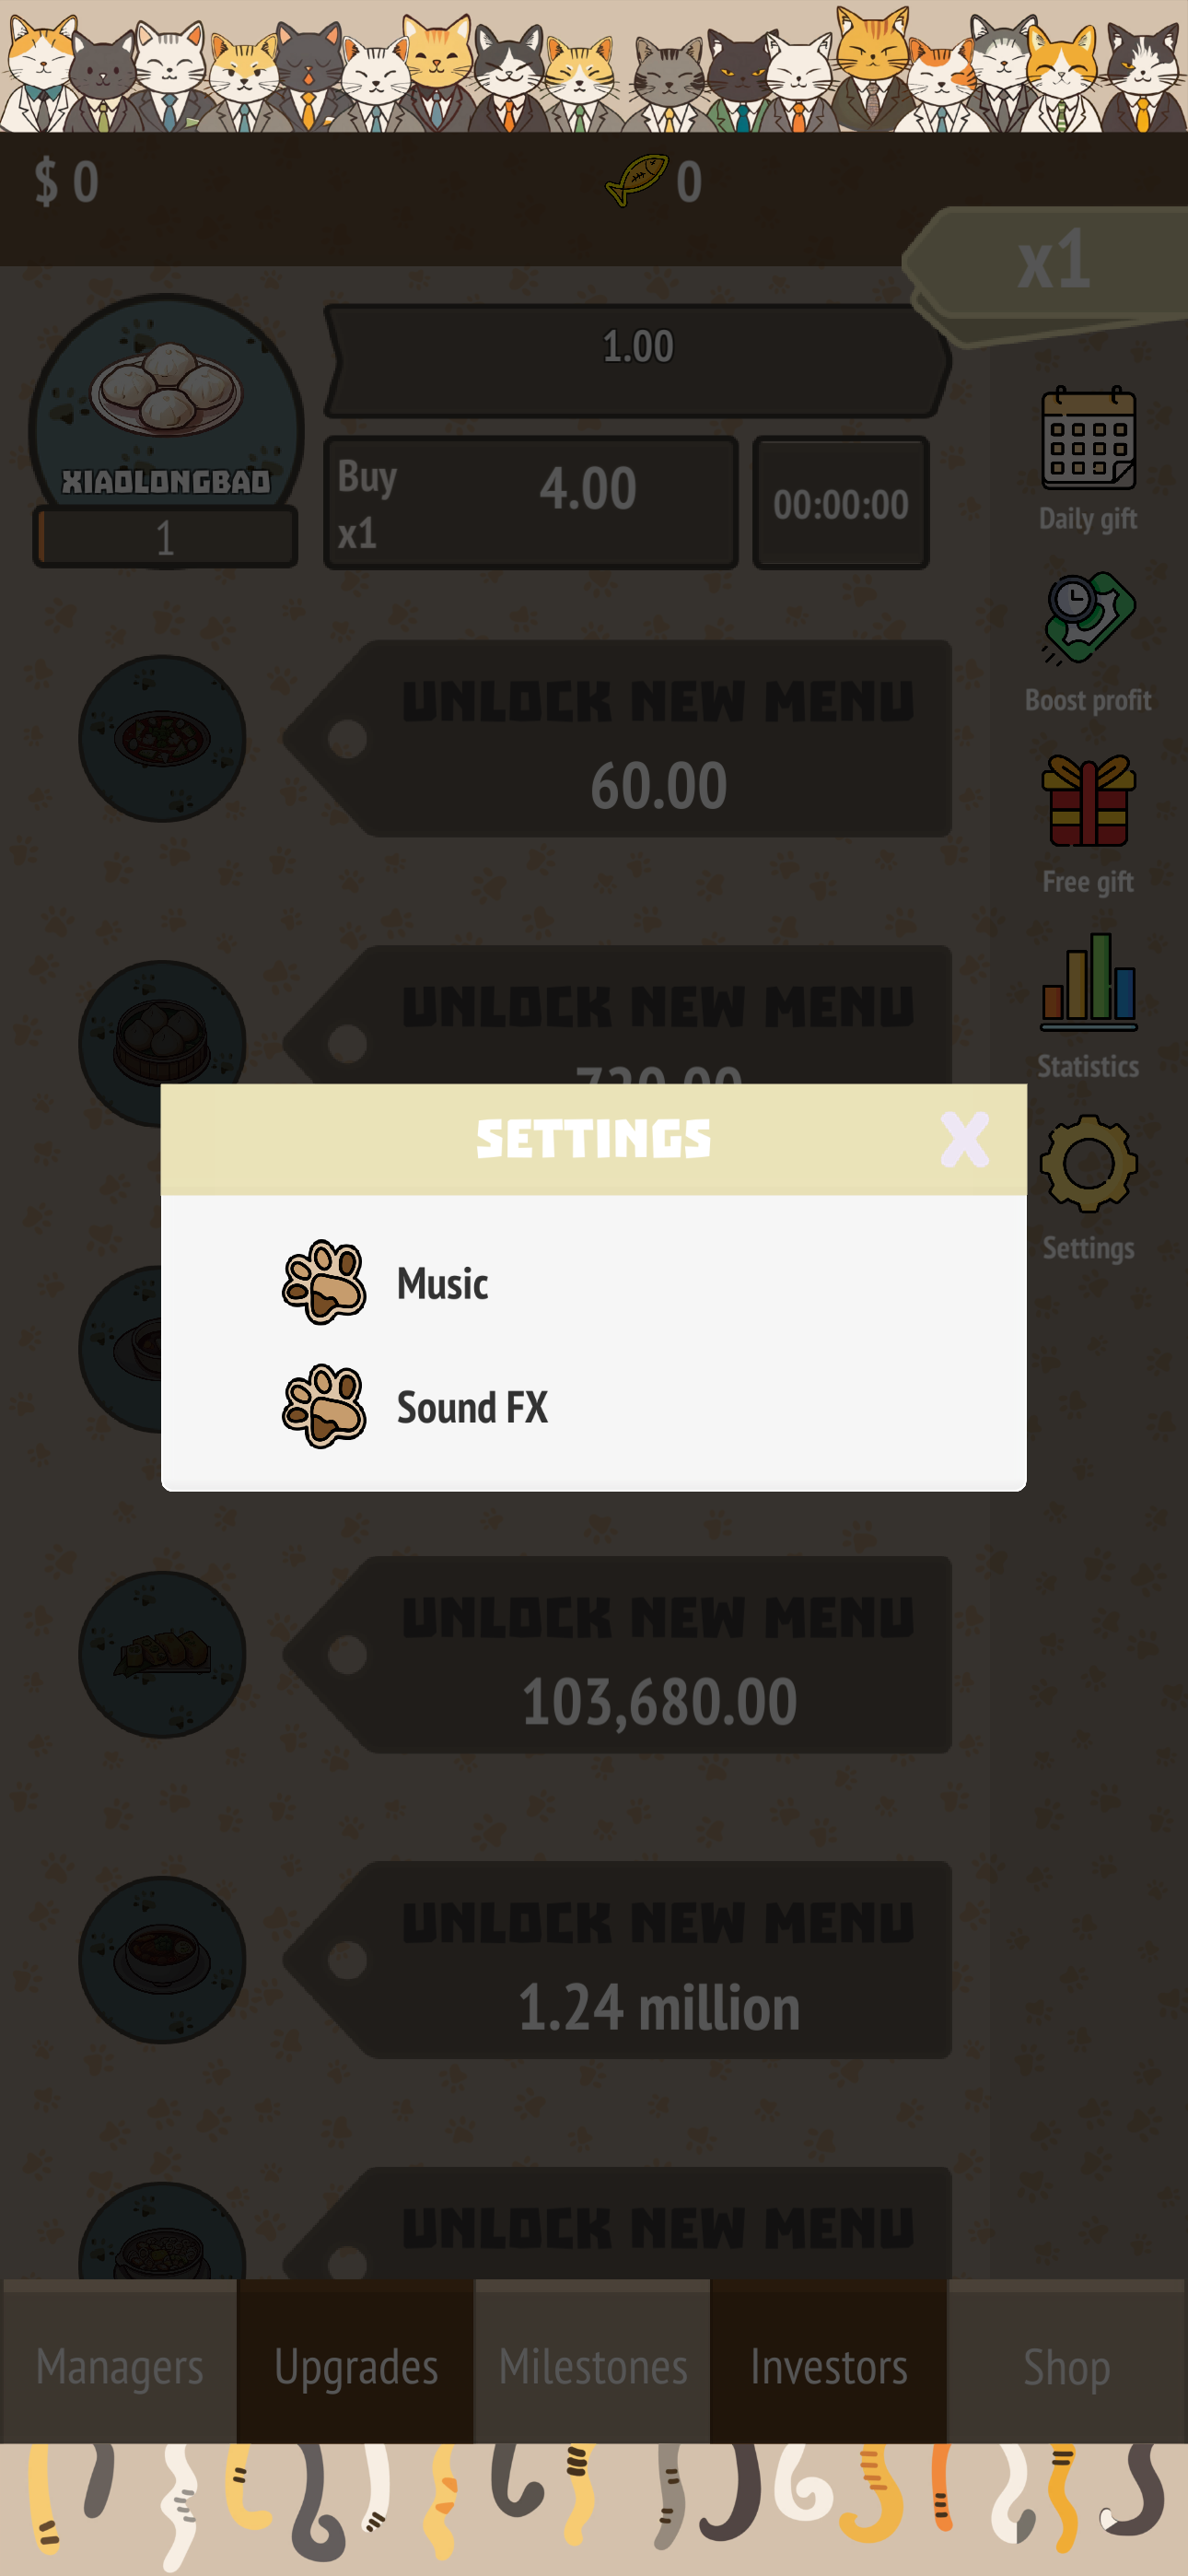
\includegraphics[height=0.6\textheight]{screenshots/PurrfectEats_009.png}
  \caption{设置界面}
\end{figure}

\subsection{音效和音乐设置}

在设置界面中,玩家可以调整以下选项:
\begin{itemize}
  \item \textbf{音乐(Music)}:开启或关闭游戏背景音乐。
  \item \textbf{音效(Sound FX)}:开启或关闭游戏音效。
\end{itemize}

这些设置可以帮助玩家根据自己的喜好调整游戏体验,使其更加舒适和愉快。
\pagebreak
\section{规范文件}

\subsection{开发规范}

开发过程中需要遵循以下规范:
\begin{itemize}
  \item 代码风格:使用统一的代码风格,确保代码的可读性和维护性。
  \item 注释规范:重要逻辑和函数必须添加注释,描述其功能和使用方法。
\end{itemize}

\subsection{编码规范}

\begin{itemize}
  \item 变量命名:使用有意义的变量名,遵循驼峰命名法。
  \item 函数命名:函数名应能描述其功能,遵循驼峰命名法。
\end{itemize}

\subsection{测试规范}

\begin{itemize}
  \item 单元测试:每个功能模块需编写相应的单元测试,确保其正确性。
  \item 集成测试:在功能集成后进行集成测试,确保各模块之间的协作正常。
\end{itemize}

\end{document} % This is the end of the document